\setbeamercovered{transparent}

\begin{document}

% -------------------------------------------------------------------------------
% -------------------------------------------------------------------------------

\begin{frame}[plain]
  
\titlepage

\end{frame}

% -------------------------------------------------------------------------------
% -------------------------------------------------------------------------------

\subtitle[Outline]{Outline}

\begin{frame}{Outline}
    \begin{itemize}
        \item Motivation
        \item \epto{} explained
        \item \sys
        \item Evaluation
        \item Conclusion
    \end{itemize}
\end{frame}

\section{Introduction}
\subtitle[Introduction]{Introduction}

\begin{frame}{Motivation}
    \epto{} was only evaluated using a \textbf{simulation}. We need an evaluation with real peers to:
    \begin{itemize}
    	\item Expose possible \textbf{limitations}
    	\item Confirm simulation \textbf{results}
    \end{itemize} 
\end{frame}

\begin{frame}{Motivation}
  \begin{itemize}
  \item Comparing \epto{} meant testing it against other algorithms
  \item No framework to easily benchmark algorithms without having to rewrite them
  \end{itemize}

\end{frame}

\subtitle[Description]{Description}

\begin{frame}{What is \epto{}?}
	\textbf{Epidemic Total Order Algorithm:}
	\begin{itemize}
		\item Probabilistic dissemination algorithm
			\begin{itemize}
				\item Using balls-and-bins
			\end{itemize}
		\item Provides deterministic total order,  integrity and validity
		\item Scales well with the number of peers
			\begin{itemize}
				\item Parameters increase logarithmically
			\end{itemize}
		\item Churn resistant
	\end{itemize}
\end{frame}

%\begin{frame}{What is \epto{}? (2)}
%	\textbf{Properties satisfied:}
%\begin{itemize}
%	\item Integrity
%	\item Validity
%	\item Total Order
%	\item Probabilistic Agreement
%\end{itemize}
%\end{frame}

%\begin{frame}{Properties satisfied}
%	\begin{itemize}
%		\item Integrity
%		\item Validity
%		\item Total Order
%		\item Probabilistic Agreement
%	\end{itemize}
%\end{frame}
\begin{frame}{\epto{} architecture}
    \begin{figure}
        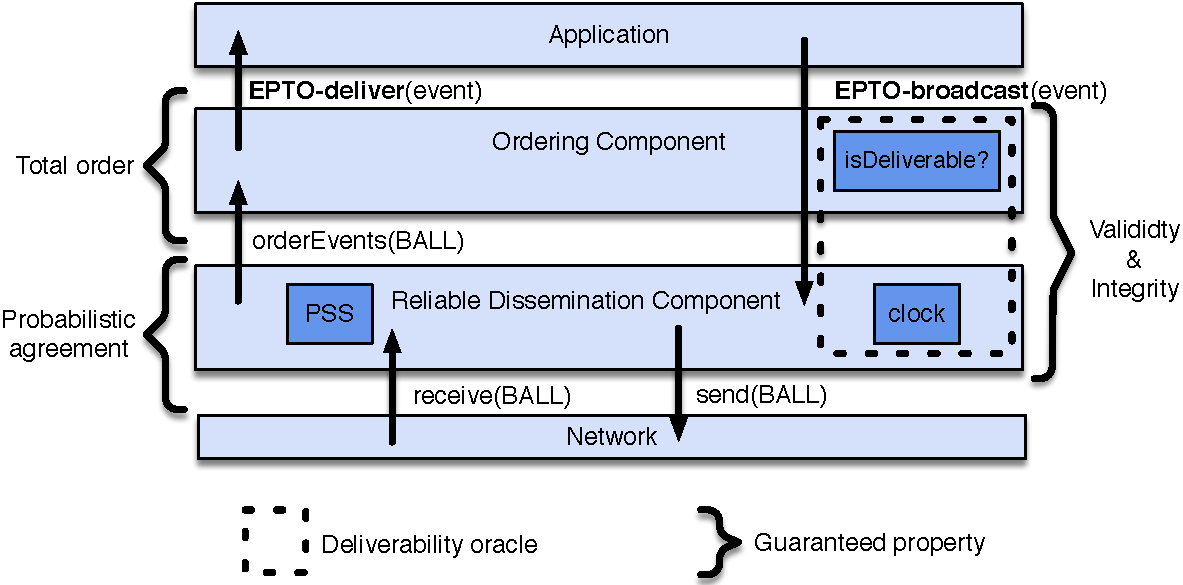
\includegraphics[scale=0.5]{figures/architecture}
    \end{figure}
\tiny{M. Matos, H. Mercier, P. Felber, R. Oliveira and J. Pereira, “EpTO: An epidemic total order algorithm for Large-scale distributed systems”, in Proceedings of the 16th Annual Middleware Conference, ACM, 2015, pp. 100–111.
}
\end{frame}

\begin{frame}{\sys{} features}
    \begin{itemize}
    	\item Compatible with any distributed algorithm provided it runs on Docker
    	\item support for a user-provided tracker
    	\item Automated benchmarking execution
    	\item Containers allow for more than 1 peer per physical node
    	\item Can simulate churn or follow real traces
    \end{itemize}
\end{frame}

\begin{frame}{\sys{} architecture}
	\begin{figure}
		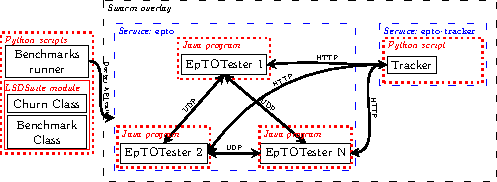
\includegraphics[scale=1.2]{complete-architecture}
	\end{figure}
\end{frame}

\begin{frame}{\sys{} Configuration and Logging}
	The protocol, churn and framework configuration is done through \textsc{YAML} files
	
	The protocols logs must be written in a file to be extracted to the host
\end{frame}

\section{Evaluation}
\subtitle[Evaluation]{Evaluation}

\begin{frame}{Evaluation}
    We evaluate \epto{} against \jgroups{} SEQUENCER, scaling peers and global event throughput per second.
    
    We write $(n,e)$ where $n$ is the number of peers and $e$ is the global event throughput per second.
\end{frame}

\begin{frame}{Bandwidth}
	\begin{figure}
		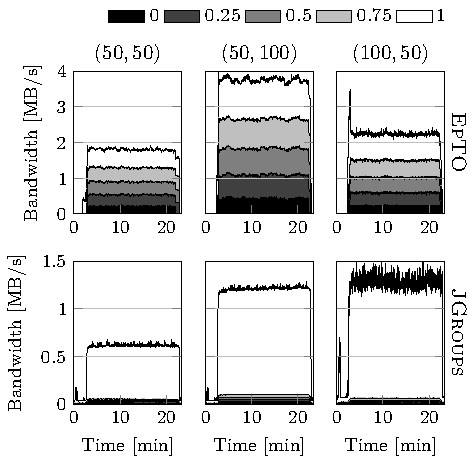
\includegraphics[scale=0.9]{bandwidth-nochurn}
	\end{figure}
\end{frame}

\begin{frame}{Bandwidth Synthetic Churn $(100,50)$}
	\begin{figure}
		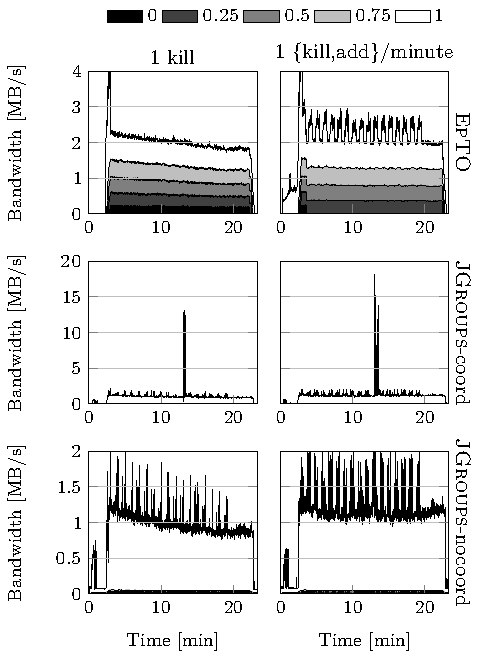
\includegraphics[scale=0.68]{bandwidth-synth-churn}
	\end{figure}
\end{frame}

\begin{frame}{Bandwidth Real Churn}
	\begin{figure}
		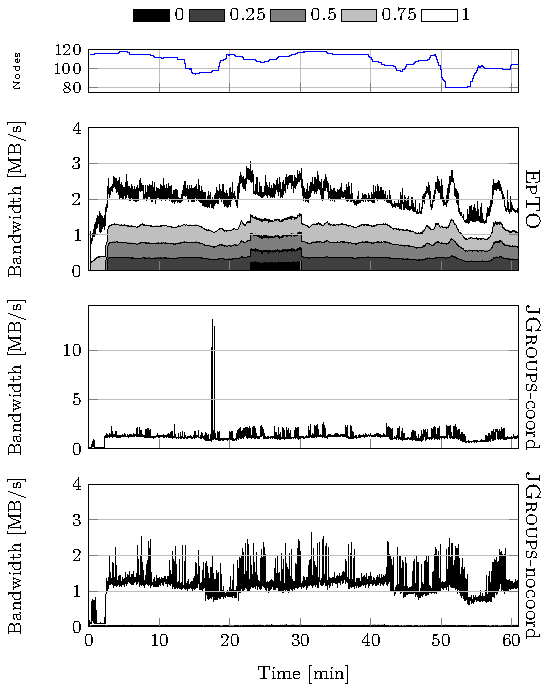
\includegraphics[scale=0.65]{bandwidth-real-churn}
	\end{figure}
\end{frame}

\begin{frame}{Local Dissemination Stretch}
	\begin{figure}
		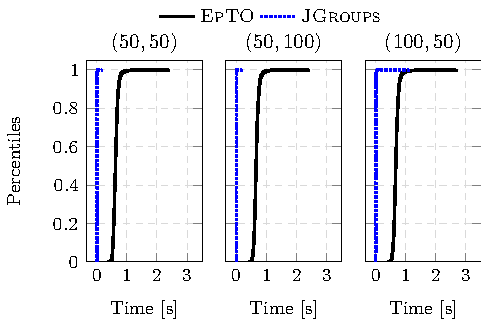
\includegraphics[scale=1]{local-diss-stretch-nochurn}
	\end{figure}
\end{frame}

\begin{frame}{Local Dissemination Stretch Synthetic Churn $(100,50)$}
	\begin{figure}
		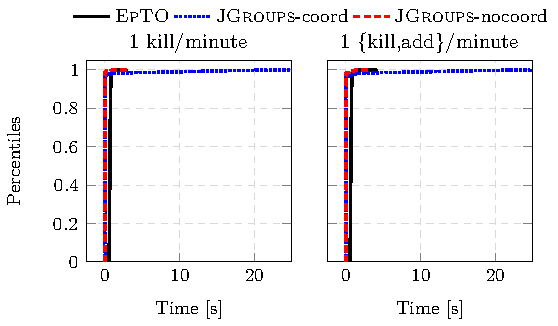
\includegraphics[scale=1]{local-diss-stretch-synth-churn}
	\end{figure}
\end{frame}

\begin{frame}{Local Dissemination Stretch Real Churn}
	\begin{figure}
		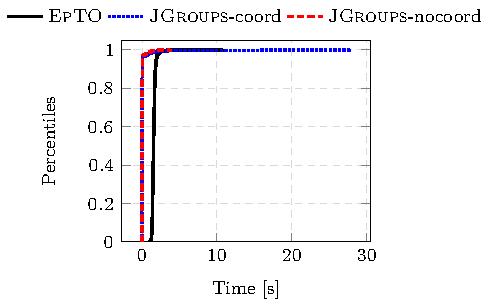
\includegraphics[scale=1]{local-diss-stretch-real-churn}
	\end{figure}
\end{frame}

\begin{frame}{Local Times}
	\begin{figure}
		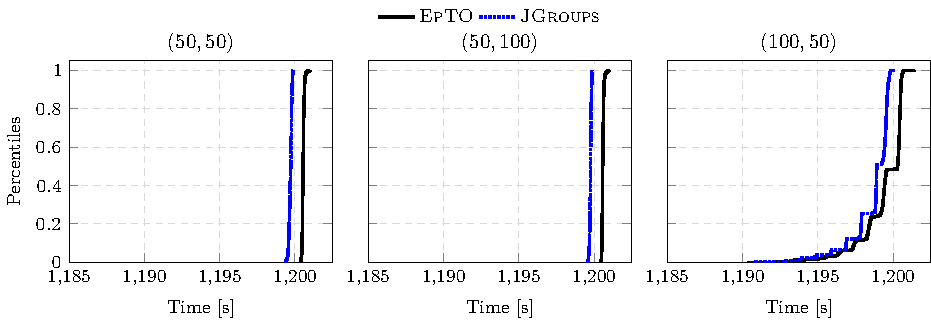
\includegraphics[scale=0.70]{local-times-nochurn}
	\end{figure}
\end{frame}

\begin{frame}{Local Times Synthetic Churn $(100,50)$}
	\begin{figure}
		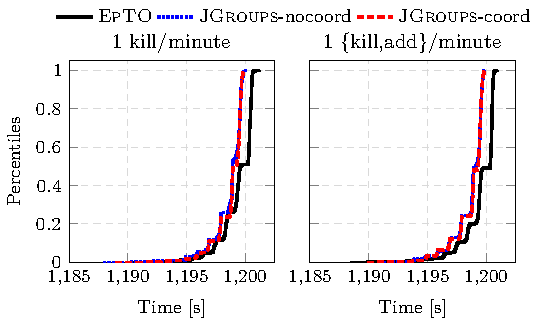
\includegraphics[scale=1]{local-times-synth-churn}
	\end{figure}
\end{frame}

\begin{frame}{Local Times Real Churn}
	\begin{figure}
		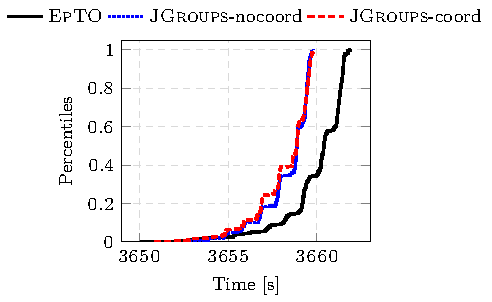
\includegraphics[scale=1]{local-times-real-churn}
	\end{figure}
\end{frame}

\begin{frame}{Total \si{\giga\byte} sent/received}
\begin{table}
	\sisetup{table-format=2.2, separate-uncertainty, table-figures-uncertainty = 2, table-align-uncertainty}
	\begin{tabular}{llSSS}
		\toprule
		&& \multicolumn{3}{c}{Cluster parameters} \\
		\cmidrule{3-5}
		{Protocol}&& {$(50,50)$} & {$(50,100)$} & {$(100,50)$} \\
		\midrule
		\multirow{2}{*}{\epto}&{Receive}& 10.84(016) & 22.31(039) & 26.01(027) \\
		&{Sending}& 10.84(016) & 22.31(039) & 26.01(027)\\
		\midrule
		\multirow{2}{*}{\jgroups}&{Receive}& 0.78(003) & 1.45(001) & 1.88(001)\\
		&{Sending}& 0.77(003) & 1.44(001) & 1.84(001)\\
		\bottomrule
	\end{tabular}
\end{table}
\end{frame}

\begin{frame}{Total events sent in a stable environment}
	\begin{table}
		\centering
		\sisetup{table-format=6.1, separate-uncertainty, table-figures-uncertainty = 2, table-align-uncertainty}
		\begin{tabular}{lSSS}
			\toprule
			& \multicolumn{3}{c}{Cluster parameters} \\
			\cmidrule{2-4}
			Protocol & {$(50,50)$} & {$(50,100)$} & {$(100,50)$} \\
			\midrule
			\epto & 59993.8(33) & 119898.2(97) & 59913.0(1643) \\
			\jgroups & 59961.9(109) & 119885.7(50) & 60023.1(2871) \\
			\bottomrule
		\end{tabular}
	\end{table}
\end{frame}

\begin{frame}{Total events sent with a synthetic churn $(100,50)$}
	\begin{table}
		\centering
		\sisetup{table-format=6.1, separate-uncertainty, table-figures-uncertainty = 2, table-align-uncertainty}
		\begin{tabular}{lSSS}
			\toprule
			& \multicolumn{2}{c}{Cluster parameters} \\
			\cmidrule{2-3}
			Protocol & {1 kill/minute} & {1\{kill,add\}/minute} \\
			\midrule
			\epto & 53898.5(1339) & 59798.6(1401) \\
			\jgroups-coord & 53834.7(1755) & 59507.9(2409) \\
			\jgroups-nocoord & 53830.5(2003) & 59450.5(1751) \\
			\bottomrule
		\end{tabular}
	\end{table}
\end{frame}

\begin{frame}{Total events sent during a real trace}
	\begin{table}
		\centering
		\sisetup{table-format=6.1, separate-uncertainty, table-figures-uncertainty = 6, table-align-uncertainty}
		\begin{tabular}{lS}
			\toprule
			Protocol & {Events sent}\\
			\midrule
			\epto & 165844.2(2102)\\
			\jgroups-coord & 166183.0(13681)\\
			\jgroups-nocoord & 166585.8(8249)\\
			\bottomrule
		\end{tabular}
	\end{table}
\end{frame}

\section{Conclusion}
\subtitle[Conclusion]{Conclusion}

\begin{frame}{Limitations}
	\begin{itemize}
		\item Difference not strong enough at 100 peers scale
		\item High CPU usage
		\item Docker problems on AWS/GCE
	\end{itemize}
\end{frame}

\begin{frame}{Future Work}
    \begin{itemize}
        \item Obtain more resources to have stronger results
        \item Implement a Push-Pull \epto{} version
        \item Use Kubernetes instead of Docker + Docker swarm
        \item Refine Framework Architecture
    \end{itemize}
\end{frame}

\begin{frame}[standout]
	Questions?
\end{frame}

\appendix

\begin{frame}{Total \si{\giga\byte} sent/received Synthetic Churn $(100,50)$}
	\begin{table}
		\centering
		\sisetup{table-format=2.2, separate-uncertainty, table-figures-uncertainty = 2, table-align-uncertainty}
		\begin{tabular}{lSSS}
			\toprule
			&& \multicolumn{2}{c}{Churn parameters} \\
			\cmidrule{3-4}
			{Protocol}&& {1 kill/minute} & {1\{kill,add\}/minute} \\
			\midrule
			\multirow{2}{*}{\epto}&{Receive}& 21.00(024) & 26.32(032)\\
			&{Sending}& 21.21(025) & 26.57(032)\\
			\midrule
			\multirow{2}{*}{\jgroups-coord}&{Receive}& 1.47(002) & 1.75(002)\\&{Sending}& 1.43(002) & 1.70(002)\\
			\midrule
			\multirow{2}{*}{\jgroups-nocoord}&{Receive}& 1.45(001) & 1.73(002)\\&{Sending}& 1.41(001) & 1.68(002)\\
			\bottomrule
		\end{tabular}
	\end{table}
\end{frame}

\begin{frame}{Total \si{\giga\byte} sent/received Real Churn}
	\begin{table}[hpt]
		\centering
		\sisetup{table-format=2.2, separate-uncertainty, table-figures-uncertainty = 2, table-align-uncertainty}
		\begin{tabular}{lSS}
			\toprule
			&& \multicolumn{1}{c}{Churn parameters} \\
			\cmidrule{3-3}
			{Protocol}&& {Real Trace} \\
			\midrule
			\multirow{2}{*}{\epto}&{Receive}& 81.41(108)\\
			&{Sending}& 82.67(108)\\
			\midrule
			\multirow{2}{*}{\jgroups-coord}&{Receive}& 5.56(008)\\
			&{Sending}& 5.40(008)\\
			\midrule
			\multirow{2}{*}{\jgroups-nocoord}&{Receive}& 5.58(005)\\
			&{Sending}& 5.43(005)\\
			\bottomrule
		\end{tabular}
	\end{table}
\end{frame}

\begin{frame}{Global Times}
	\begin{figure}
		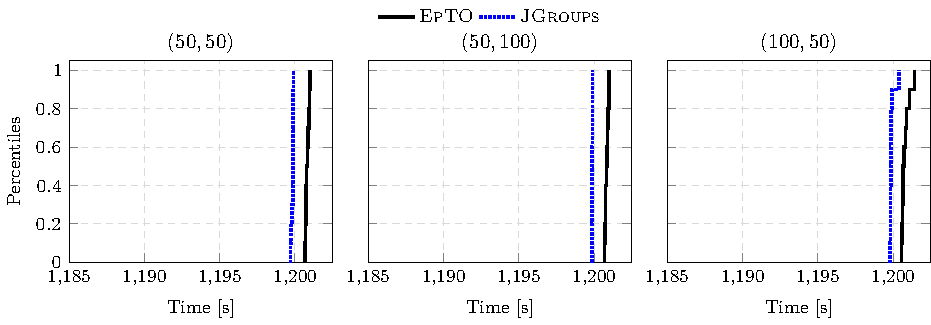
\includegraphics[scale=0.65]{global-times-nochurn}
	\end{figure}
\end{frame}

\begin{frame}{Global Times Synthetic Churn}
	\begin{figure}
		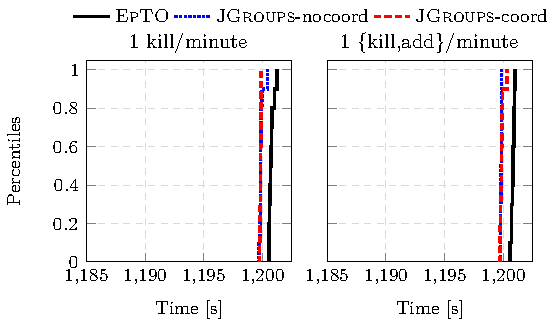
\includegraphics[scale=1]{global-times-synth-churn}
	\end{figure}
\end{frame}

\begin{frame}{Global Times Real Churn}
	\begin{figure}
		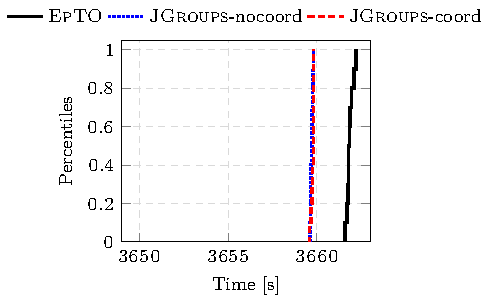
\includegraphics[scale=1]{global-times-real-churn}
	\end{figure}
\end{frame}

% -------------------------------------------------------------------------------
% -------------------------------------------------------------------------------

\end{document}

% -------------------------------------------------------------------------------
